\documentclass[11pt]{article}
\usepackage{tikz, pgfplots}
\tikzstyle{circleblock} = [draw, fill=white, circle, node distance=0.1cm]
\usetikzlibrary{arrows.meta}

\begin{document}
  \begin{figure}[!htbp]
    \centering
    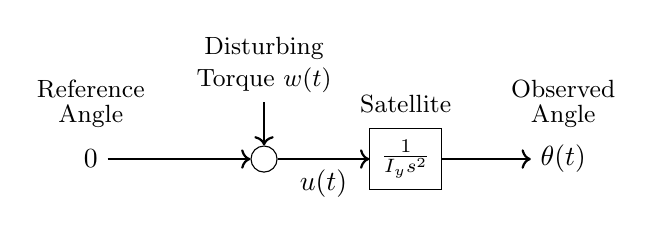
\begin{tikzpicture}
      \node (ref) at (8, 0) {$0$};
      \node at (8, 0.7) {\shortstack{\small Reference \\ \small Angle}};
      \node[circleblock] (sum2) at (10.2, 0) {};
      \node (disturb) at (10.2, 1.2) {\shortstack{\small Disturbing \\ \small Torque $w(t)$}};
      \node[draw, inner sep=4pt] (vehicle) at (12, 0) {$\frac{1}{I_y s^2}$};
      \node (theta) at (14, 0) {$\theta(t)$};
      \node at (14, 0.7) {\shortstack{\small Observed \\ \small Angle}};
      \node at (12, 0.7) {\small Satellite};
      \draw[->, thick] (ref) -- (sum2);
      \draw[->, thick] (disturb) -- (sum2);
      \draw[->, thick] (sum2) -- node[below] {$u(t)$} (vehicle);
      \draw[->, thick] (vehicle) -- (theta);
    \end{tikzpicture} \\[20pt]
    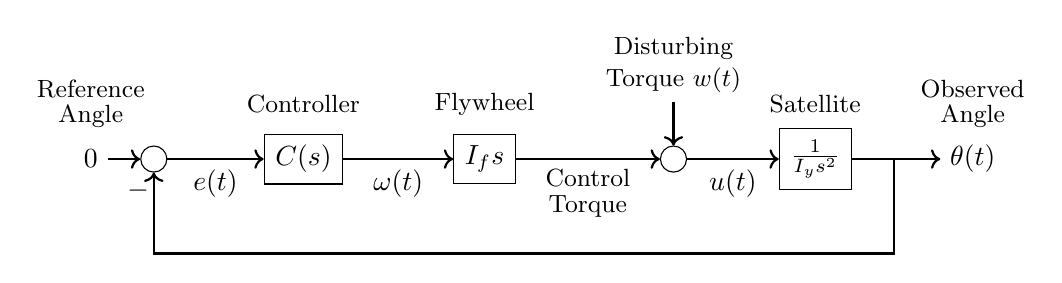
\begin{tikzpicture}
      \node (ref) at (2.8, 0) {$0$};
      \node at (2.8, 0.7) {\shortstack{\small Reference \\ \small Angle}};
      \node[circleblock] (sum1) at (3.6, 0) {};
      \node[draw, inner sep=4pt] (controller) at (5.5, 0) {$C(s)$};
      \node at (5.5, 0.7) {\small Controller};
      \node[draw, inner sep=4pt] (flywheel) at (7.8, 0) {$I_f s$};
      \node at (7.8, 0.7) {\small Flywheel};
      \node[circleblock] (sum2) at (10.2, 0) {};
      \node (disturb) at (10.2, 1.2) {\shortstack{\small Disturbing \\ \small Torque $w(t)$}};
      \node[draw, inner sep=4pt] (vehicle) at (12, 0) {$\frac{1}{I_y s^2}$};
      \node (theta) at (14, 0) {$\theta(t)$};
      \node at (14, 0.7) {\shortstack{\small Observed \\ \small Angle}};
      \node at (12, 0.7) {\small Satellite};
      \node at (3.4, -0.4) {$-$};

      \draw[->, thick] (ref) -- (sum1);
      \draw[->, thick] (sum1) -- node[below] {$e(t)$} (controller);
      \draw[->, thick] (controller) -- node[below] {$\omega(t)$} (flywheel);
      \draw[->, thick] (flywheel) -- node[below] {\shortstack{\small Control\\ \small Torque}} (sum2);
      \draw[->, thick] (disturb) -- (sum2);
      \draw[->, thick] (sum2) -- node[below] {$u(t)$} (vehicle);
      \draw[->, thick] (vehicle) -- (theta);
      \draw[->, thick] (13, 0) -- (13, -1.2) -- (3.6, -1.2) -- (sum1);
    \end{tikzpicture} \\[20pt]
    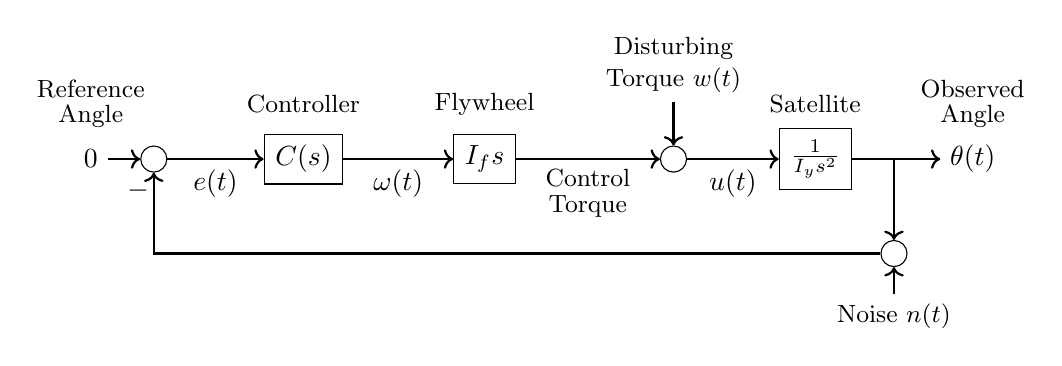
\begin{tikzpicture}
      \node (ref) at (2.8, 0) {$0$};
      \node at (2.8, 0.7) {\shortstack{\small Reference \\ \small Angle}};
      \node[circleblock] (sum1) at (3.6, 0) {};
      \node[draw, inner sep=4pt] (controller) at (5.5, 0) {$C(s)$};
      \node at (5.5, 0.7) {\small Controller};
      \node[draw, inner sep=4pt] (flywheel) at (7.8, 0) {$I_f s$};
      \node at (7.8, 0.7) {\small Flywheel};
      \node[circleblock] (sum2) at (10.2, 0) {};
      \node (disturb) at (10.2, 1.2) {\shortstack{\small Disturbing \\ \small Torque $w(t)$}};
      \node[draw, inner sep=4pt] (vehicle) at (12, 0) {$\frac{1}{I_y s^2}$};
      \node (theta) at (14, 0) {$\theta(t)$};
      \node at (14, 0.7) {\shortstack{\small Observed \\ \small Angle}};
      \node at (12, 0.7) {\small Satellite};
      \node[circleblock] (sum3) at (13, -1.2) {};
      \node (noise) at (13, -2) {\small Noise $n(t)$};
      \node at (3.4, -0.4) {$-$};

      \draw[->, thick] (ref) -- (sum1);
      \draw[->, thick] (sum1) -- node[below] {$e(t)$} (controller);
      \draw[->, thick] (controller) -- node[below] {$\omega(t)$} (flywheel);
      \draw[->, thick] (flywheel) -- node[below] {\shortstack{\small Control\\ \small Torque}} (sum2);
      \draw[->, thick] (disturb) -- (sum2);
      \draw[->, thick] (sum2) -- node[below] {$u(t)$} (vehicle);
      \draw[->, thick] (vehicle) -- (theta);
      \draw[->, thick] (13, 0) -- (sum3);
      \draw[->, thick] (noise) -- (sum3);
      \draw[->, thick] (sum3) -- (3.6, -1.2) -- (sum1);
    \end{tikzpicture} \\[20pt]
    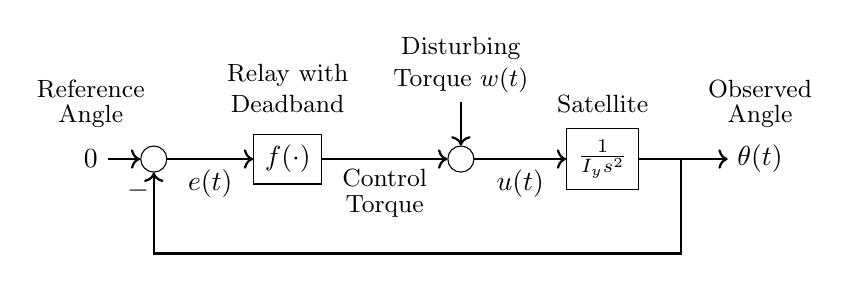
\begin{tikzpicture}
      \node (ref) at (5.5, 0) {$0$};
      \node at (5.5, 0.7) {\shortstack{\small Reference \\ \small Angle}};
      \node[circleblock] (sum1) at (6.3, 0) {};
      \node[draw, inner sep=4pt] (controller) at (8, 0) {$f(\cdot)$};
      \node at (8, 0.9) {\shortstack{\small Relay with \\ \small Deadband}};
      \node[circleblock] (sum2) at (10.2, 0) {};
      \node (disturb) at (10.2, 1.2) {\shortstack{\small Disturbing \\ \small Torque $w(t)$}};
      \node[draw, inner sep=4pt] (vehicle) at (12, 0) {$\frac{1}{I_y s^2}$};
      \node (theta) at (14, 0) {$\theta(t)$};
      \node at (14, 0.7) {\shortstack{\small Observed \\ \small Angle}};
      \node at (12, 0.7) {\small Satellite};
      \node at (6.1, -0.4) {$-$};

      \draw[->, thick] (ref) -- (sum1);
      \draw[->, thick] (sum1) -- node[below] {$e(t)$} (controller);
      \draw[->, thick] (controller) -- node[below] {\shortstack{\small Control\\ \small Torque}} (sum2);
      \draw[->, thick] (disturb) -- (sum2);
      \draw[->, thick] (sum2) -- node[below] {$u(t)$} (vehicle);
      \draw[->, thick] (vehicle) -- (theta);
      \draw[->, thick] (13, 0) -- (13, -1.2) -- (6.3, -1.2) -- (sum1);
    \end{tikzpicture} \\[20pt]
    \begin{tikzpicture}
      \begin{axis}[axis lines=middle, xlabel=$e$, ylabel=$f(e)$, width=0.6\textwidth, height=0.4\textwidth, xtick={1}, xticklabels={$+\delta$}, ytick={-1, 1}, yticklabels={$-\tau$, $+\tau$}, ymax=1.2, extra x ticks={-1}, extra x tick labels={$-\delta$}, extra x tick style={tick label style={above, yshift=0.4em}}]
        \addplot[thick] plot coordinates {(-2, -1) (-1, -1)};
        \addplot[thick, dashed] plot coordinates {(-1, -1) (-1, 0)};
        \addplot[thick] plot coordinates {(-1, 0) (1, 0)};
        \addplot[thick, dashed] plot coordinates {(1, 0) (1, 1)};
        \addplot[thick] plot coordinates {(1, 1) (2, 1)};
      \end{axis}
    \end{tikzpicture}
  \end{figure}
\end{document}
